\chapter{Firewall}

For ACL, take a look at chapter ACL in Notebook folder.\\

All firewalls share some common properties: resistant to attacks, the only transit point between networks because all traffic flows through the firewall, enforce the access control policy. 

\section{Firewall types}

\subsection{Packet filtering}

Basic packet filtering firewalls can only filter based on Layer 3 and sometimes basic Layer 4 information. \\

\textbf{Benefits:} Simple implementation, Low impact on network performance, Initial degree of security at the network layer, Almost all the tasks of a high-end firewall at a much lower cost.\\

\textbf{Limitations:} Susceptible to IP spoofing, Not reliably filter fragmented packets, Complex ACLs (difficult to implement and maintain), \emph{Stateless:} examine each packet individually rather than in the context of the state of a connection.

\subsection{Statefull firewall}

Stateful firewall monitors network traffic as it flows into and out of the organization and determines whether packets belong to an existing connection or are from an unauthorized source. Stateful filtering tracks each connection and confirms that they are valid. Stateful firewalls use a state table to keep track of the actual communication process.\\ 

\textbf{Benefits:} Prevent spoofing and DoS attacks; Provide more control over security.\\ 

\textbf{Limitations:} Cannot prevent UDP, ICMP, and layer 7 attacks; No authentication; Cannot detect dynamic port negotiation.

\subsection{Next-Generation Firewall}

Designed with advanced malware protection, the Cisco ASA with FirePOWER services is also called the \textbf{Cisco ASA Next-Generation Firewall} because it is an adaptive, threat-focused firewall. It is designed to provide defense across the entire attack continuum, which includes before, during, and after attacks.

\subsection{DMZ}

A demilitarized zone (DMZ) is a firewall design where there is typically one inside interface connected to the private network, one outside interface connected to the public network, and one DMZ interface, as shown in the figure \ref{DMZfilter}.

\begin{figure}[hbtp]
\caption{DMZ topology and traffic restriction}\label{DMZfilter}
\centering
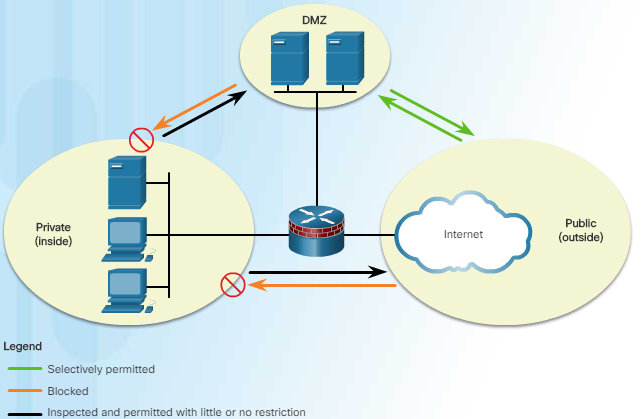
\includegraphics[width=10\xm]{pictures/DMZfilter.PNG}
\end{figure}

\begin{itemize}
\item Private network $\rightarrow$ DMZ: Inspected 
\item DMZ  $\rightarrow$ Private network: Blocked
\item Public network  $\leftrightarrow$ DMZ: selectively permitted
\item Private network $\rightarrow$ Public network: Inspected
\item Public network $\rightarrow$ Private network: Blocked
\end{itemize}

\subsection{Layered Defense}

A layered defense uses different types of firewalls that are combined in layers. Security policies can be enforced between the layers and inside the layers. A traffic from the untrusted network has to go through the following layers and policies:

\begin{enumerate}
\item Edge router (packet filtering)
\item Bastion host (hardened computer located in the DMZ\footnote{This type of DMZ setup is called a \emph{screened subnet configuration}.}) or Screened firewall
\item Interior screening router
\end{enumerate}

\section{Cisco firewall}

There are two configuration models for Cisco IOS Firewall: \hyperref[sec:ClassicFirewall]{Classic Firewall} and \hyperref[sec:ZPF]{Zone-based Policy Firewall (ZPF)}.

\subsection{Classic firewall}\label{sec:ClassicFirewall}

Classic Firewall (CBAC) is a \emph{stateful} firewall that provides four main functions: Filtering, Inspection, Intrusion detection, and Generation of audits and alerts. It can only detects and protects against external attacks. \emph{The Classic Firewall applies firewall policy to interfaces.}\\ 

Classic Firewall creates \emph{temporary} openings in the ACL to allow returning traffic. These entries are created as inspected traffic leaves the network and are removed when the connection terminates or the idle timeout period for the connection is reached. 
In addition to extended ACLs, Application layer protocol session information is used by a classic firewall to filter traffic. Figure \ref{ClassicFirewall} shows how Classic Firewall inspects SSH traffic.

\begin{figure}[hbtp]
\caption{Classic Firewall inspects SSH traffic}\label{ClassicFirewall}
\centering
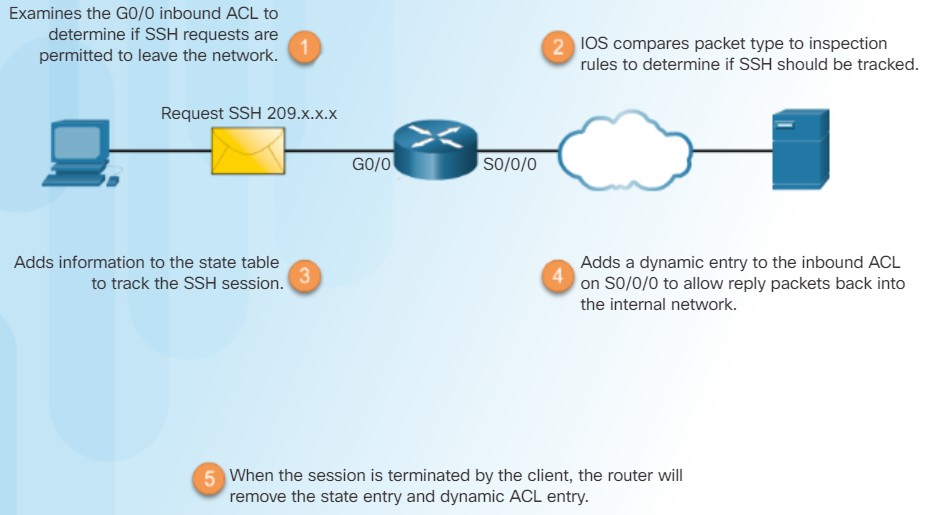
\includegraphics[ width=10\xm ]{pictures/ClassicFirewall.PNG}
\end{figure}

Take the topology in figure \ref{ClassicConfig} as an example for configuration. Suppose that the administrator wants to allow SSH sessions between the 10.0.0.0 and 172.30.0.0 networks. However, only hosts from the 10.0.0.0 network are allowed to initiate SSH sessions. All other access is denied. 

\begin{figure}[hbtp]
\caption{Network topology}\label{ClassicConfig}
\centering
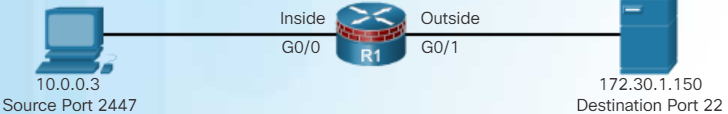
\includegraphics[width=10\xm]{pictures/ClassicConfig.PNG}
\end{figure}


\begin{sexylisting}{Classic Firewall configuration}
ip access-list extended INSIDE
  permit tcp 10.0.0.0 0.0.0.255 any eq 22
ip access-list extended OUTSIDE
  deny ip any any

ip inspect name FWRULE ssh

interface g0/0
  ip access-group INSIDE in
  ip inspect FWRULE in
interface g0/1
  ip access-group OUTSIDE in
\end{sexylisting}

There are four steps to configure this policy using a Classic Firewall:

\begin{enumerate}
\item \textbf{Define the internal and external interfaces}: G0/0 is the inside interface and G0/1 is the outside interface.
\item \textbf{Configure ACLs for each interface}: The INSIDE ACL allows only SSH traffic from the 10.0.0.0 network; the OUTSIDE ACL will deny inbound traffic from the 172.30.0.0 network.
\item \textbf{Define inspection rules}: The inspection rule FWRULE specifies that traffic will be inspected for SSH connections. This inspection rule has no effect until it is applied to an interface.
\item \textbf{Apply an inspection rule to an interface}: When the FWRULE is applied to inbound traffic on the G0/0 interface, the Classic Firewall configuration will dynamically add an entry to allow inbound SSH traffic from the 172.30.0.0 network. From now on, the FWRULE inspects SSH traffic between 10.0.0.0 and 172.30.0.0 network.
\item \textbf{Verification}: Use \code{show ip inspect sessions} command to verify inspect sessions.
\end{enumerate}

\section{Zone-based Policy Firewall (ZPF)}\label{sec:ZPF}

\subsection{Introduction}

\emph{Zone-Based Policy Firewall applies firewall policy to zones.} A zone is a group of one or more interfaces. \\

By default, the traffic between interfaces in the same zone passes freely. However, all zone-to-zone traffic is blocked. In order to permit traffic between zones, a ZPF policy must be applied on each zone.\\

The only exception to this default deny any policy is the router \textbf{self zone}. The self zone is the router itself and includes all the router interfaces. Policy configurations that include the self zone would apply to traffic destined to and sourced from the router. By default, there is no policy for this type of traffic. Traffic that should be considered when designing a policy for the self zone includes management plane and control plane traffic, such as SSH, SNMP, and routing protocols.\\

\textbf{Benefits} of a ZPF: Not dependent on ACLs, The default policy is to block unless explicitly allowed, Policies are easy to read and troubleshoot with the C3PL\footnote{Cisco Common Classification Policy Language}, which can create traffic policies based on events and it affects any given traffic with only one policy, instead of needing multiple ACLs and inspection actions.

\tableStart[\caption{Compare Classic Firewall and ZPF operation}]{| p{6\xm} | p{2\xm} | p{2\xm} |}
Only prevent attacks that travel through the firewall & $\bullet$ & \w
Require multiple ACLs and inspection actions &$\bullet$& \w
Not dependent on ACLs & & $\bullet$ \w
One policy affects any given traffic & & $\bullet$ \w
Firewall policy is applied on interfaces & $\bullet$ & \w
Firewall policy is applied on zones & & $\bullet$ \w
Examine connections for embedded NAT and PAT and perform address translation & $\bullet$ & \w
The default policy is to block unless explicitly allowed & & $\bullet$ \w
\tableEnd

\subsection{Configuration}

  If the Security Technology package has not been enabled, use the following command to enable the package: \code{license boot module c1900 technology-package securityk9}.   Accept the end-user license agreement.  Save the running-config and reload the router to enable the security license.  Verify that the Security Technology package has been enabled by using the show version command.

\subsubsection{Identify traffic using Class-Maps}

\begin{enumerate}
\item (Optional) Create an ACL that defines internal traffic. The access list shown below defines internal traffic which is  all IP protocols from the 192.168.3.0/24 source network to any destination.
\item Create class-maps using the pre-defined ACL or port numbers of protocols. In the following commands, all traffics that match access list 100 are assigned to the class-map PRIVATE-ACL-CLASS. Any HTTP, or HTTPS, or DNS traffics are assigned to the class-map PRIVATE-INTERNET-CLASS.
\end{enumerate}

\begin{sexylisting}{ZPF configuration: Identify traffic using ACLs and Class-Maps}
#STEP 1
access-list 100 permit ip 192.168.3.0 0.0.0.255 any

#STEP 2
class-map type inspect match-all PRIVATE-ACL-CLASS
  match access-group 100    
class-map type inspect match-any PRIVATE-INTERNET-CLASS
  match protocol http
  match protocol https
  match protocol dns
exit    
\end{sexylisting}

\subsubsection{Specify Firewall Policies}

\begin{enumerate}
\item Create a policy map to determine what to do with matched traffic.
\item Specify a class type of inspect and reference class map.
\item Specify the action of inspect for this policy map.
\end{enumerate}

\begin{sexylisting}{ZPF configuration: Specify Firewall Policies}
policy-map type inspect PRIV-TO-PUB-POLICY
  class type inspect PRIVATE-ACL-CLASS   
  inspect    
  class type inspect PRIVATE-INTERNET-CLASS
  inspect
  class class-default
exit  
\end{sexylisting}

\subsubsection{Apply Firewall Policies}

\begin{enumerate}
\item Create zones.
\item Create a pair of zones. The example commands below create a zone pair PRIVATE-2-INTERNET between PRIVATE and INTERNET.
\item Specify the policy map for handling the traffic between the two zones. The following commands associate that zone pair to a policy-map PRIV-TO-PUB-POLICY.
\item Assign interfaces to the appropriate security zones.
\end{enumerate}


\begin{sexylisting}{ZPF configuration: Apply Firewall Policies}
#STEP 1
zone security PRIVATE
zone security INTERNET
zone security DMZ

#STEP 2 and 3
zone-pair security PRIVATE-2-INTERNET source PRIVATE destination INTERNET
  service-policy type inspect  PRIV-TO-PUB-POLICY
end

#STEP 4
int g0/1
  zone-member security PRIVATE
int s0/0/0
  zone-member security INTERNET    
int g0/0
  zone-member security DMZ
exit
\end{sexylisting}

\subsection{Verification}

The service-policy is now active. HTTP, HTTPS, and DNS traffic sourced from the PRIVATE zone and destined for the PUBLIC zone will be inspected. Traffic sourced from the PUBLIC zone and destined for the PRIVATE zone will only be allowed if it is part of sessions originally initiated by PRIVATE zone hosts.

\begin{sexylisting}{ZPF Verification}
show run | begin class-map
show class-map type inspect
show zone security
show zone-pair security
show policy-map type inspect
show policy-map type inspect zone-pair sessions
\end{sexylisting}


%
%There are four steps to configure a ZPF zone (Take the topology in figure \ref{Zone} as an example):
%
%\begin{enumerate}
%\item \textbf{Create the zones and Assign zones to appropriate interfaces:} Associating a zone to an interface will immediately apply the service-policy that has been associated with the zone. If no service-policy is yet configured for the zone, all transit traffic will be dropped.
%
%\item \textbf{Identify traffic with class-map:} A class is a way of identifying a set of packets based on its contents using \code{match} conditions. Packets must meet one of the match criteria \code{match-any} or all of the match criteria \code{match-all} to be considered a member of the class. Table \ref{tab:classMap} shows the syntax for the \code{class-map} and its sub-commands.
%
%\item \textbf{Define an action with policy-map:} Assign class-maps defined in step 2 to a policy-map and define what action (Inspect, Drop, or Pass) should be taken for traffic that is a member of a class. 
%\item \textbf{Identify a zone-pair and match it to a policy-map:} 
%\end{enumerate}
%
%\begin{figure}[hbtp]
%\caption{ZPF configuration topology}\label{Zone}
%\centering
%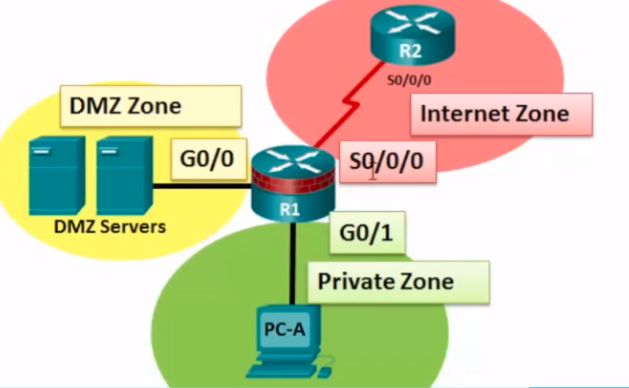
\includegraphics[scale=0.5]{pictures/Zone.PNG}
%\end{figure}
%
%\begin{sexylisting}{ZPF configuration}
%#STEP 1
%zone security PRIVATE
%zone security INTERNET
%zone security DMZ
%int g0/1
%  zone-member security PRIVATE
%int s0/0/0
%  zone-member security INTERNET    
%int g0/0
%  zone-member security DMZ
%exit
%
%#STEP 2
%class-map type inspect match-all PRIVATE-ACL-CLASS
%  match access-group 100    
%class-map type inspect match-any PRIVATE-INTERNET-CLASS
%  match protocol http
%  match protocol https
%  match protocol dns
%exit    
%
%#STEP 3
%policy-map type inspect PRIV-TO-PUB-POLICY
%  class type inspect PRIVATE-ACL-CLASS   
%  inspect    
%  class type inspect PRIVATE-INTERNET-CLASS
%  inspect
%  class class-default
%exit   
%
%#STEP 4
%zone-pair security PRIVATE-2-INTERNET source PRIVATE destination INTERNET
%  service-policy type inspect  PRIV-TO-PUB-POLICY
%end
%\end{sexylisting}

\subsection{Command syntax and some considerations}

\begin{itemize}
\item The router never filters the traffic between interfaces in the same zone.
\item An interface cannot belong to multiple zones.
ZPF can coexist with Classic Firewall although they cannot be used on the same interface. Remove the \code{ip inspect} interface configuration command before applying the \code{zone-member security} command.
\item Traffic can never flow between an interface assigned to a zone and an interface without a zone assignment. Applying the zone-member configuration command always results in a temporary interruption of service until the other zone-member is configured.
\item Communication between zones are, by default, dropped. Unless there exits a service-policy configured for the zone-pair.
\item The \code{zone-member} command does not protect the router itself (traffic to and from the router is not affected) unless the zone-pairs are configured using the predefined self zone.
\end{itemize}

\tableStart[\caption{The syntax of class-map command}\label{tab:classMap}] { |p{5\xm}|p{8\xm}| }
\multicolumn{2}{|c|}{ \code{class-map type inspect [match-any | match-all] <class-name>} } \w
\head{Parameter}&\head{Description} \w
\code{match-any} & Packets must meet one of the criteria to be considered a member of the class.\w
\code{match-all} & Packets must meet all of the criteria to be considered a member of the class.\w
\code{match protocol <protocol-name>} & Configure criteria based on specified protocol.\w
\code{match access-group <acl-name>} & Configure criteria based on specified ACL.\w
\code{match class-map <class-name>} & Use another class-map as criteria.\w
\tableEnd

\begin{itemize}
\item \code{inspect} -- This action offers state-based traffic control. It tracks UDP or TCP connections and permit the return traffic.
\item \code{drop} -- This is the default action for all traffic. Similar to the implicit deny any at the end of every ACL, , there is an explicit \code{drop} applied to the end of every policy-map.
\item \code{pass} -- This action allows \emph{one-direction} traffic between two zones, and does not track the state of connections. A corresponding policy must be applied to allow return traffic to pass in the opposite direction. This action is ideal for secure protocols, such as IPsec. 
\end{itemize}
